%Diese LaTeX-Vorlage f�r Praktikumsprotokolle in Form einer Ver�ffentlichung f�r das 
%F-Praktikum wurde erstellt von Andreas Nuber EP II, Uni W�rzburg.
%Es wurde das Koma-Skript verwendet und sollte somit installiert sein
%desweiteren sollten alle packages installiert sein, die mit \usepackage{} 
%eingebunden werden.
%Zum Testen dieser Vorlage wurde MikTex verwendet sowie TeXnicCenter als Editor
%beim Compilieren waren 0 Fehler, 1 Warnung und 3 zu volle/leere Boxen. Das ist ok :)

%F�r das Erstellen einfach den sinnfreien Text, der zum ausf�llen genommen wurde 
%ersetzen. Was sonst noch ver�ndert werden sollte steht in den Kommentaren!


\documentclass[a4paper,10pt,twocolumn]{scrartcl} %Koma-Skript-�quivalent zu "article"

\usepackage{german}            %macht deutsche �berschriften
\usepackage{amsmath}           %macht
\usepackage{amsfonts}          %       Mathe
\usepackage{amssymb}           %              m�chtiger
\usepackage{graphicx}          %erlaubt Graphiken einzubinden (.eps f�r dvi und ps sowie .jpg f�r pdf)
\usepackage[T1]{fontenc}       %Zeichenbelegung der verwendeten Schrift
\usepackage{ae}                %macht sch�neres �
\usepackage{typearea}	         %erm�glicht �nderung des Seitenspiegels
\usepackage{scrlayer-scrpage}          %erm�glicht �nderung der Kopf-/Fu�zeile
\usepackage{lastpage}         %l�sst auf die Seienanzahl zugreifen
\usepackage[margin=10pt,font=small,labelfont=bf]{caption} %macht die Bildbeschriftungen richtig
\usepackage{xcolor}			  % macht Farbe
\usepackage{subfig}
\usepackage{hyperref}
\usepackage{float}
\usepackage{comment}

\renewcommand{\figurename}{Abb.}

\pagestyle{scrheadings}        %sagt Koma-Skript, dass selbstdefiniers Kopfzeilen verwendet werden
\typearea{16}                  %stellt Seitenspiegel ein
\columnsep25pt								 %definiert Breite zwischen den zwei Spalten von \twocolumns

\renewcommand{\pnumfont}{%     %�ndert die Schriftart der Seitennummerierung
\normalfont\rmfamily\slshape}  %�ndert die Schriftart der Seitennummerierung 



\begin{document}
\cfoot{\thepage /\pageref{LastPage}}     %macht die Seitennumerierung der Fom 2/5 (ausser auf der Titelseite)

\twocolumn[{\csname @twocolumnfalse\endcsname                %erlaubt "Abstrakt" �ber beide Spalten
\titlehead{                                                  %Kopfzeile
	\begin{tabular*}{\textwidth}[]{@{\extracolsep{\fill}}lr}   %Kopfzeile
	Betreuer: Prof. Dr. V. Hinkov & \today\\                          %Kopfzeile      hier den Betreuer eintragen!!!
	\end{tabular*}                                             %Kopfzeile
	}
\title{Plancksches Wirkungsquantum und Boltzmann-Konstante}  %Titel der Versuchs
\author{Hannes Winkler \and Moritz Langer}                     %Namen der Studenten
\date{}			                                               %ben�tigt um automatisches Datum auszuschalten
\maketitle                                                      %erzeugt Titelseite
\vspace{-8ex}                                                   %verringert Abstand zur �berschrift
\begin{abstract}                                                %Beginn des Abstracts
\vspace{1em}
\noindent Versuchsdurchführung: 20. November 2025\\% Datum ändern!
\noindent Protokollabgabe: 4. Dezember 2025% Datum ändern!
\vspace{1em}

	\noindent abstrahiertes abstract
\end{abstract}
}]

\section{Einleitung}
	Dieser Versuch beschäftigt sich mit dem Plankschen Wirkungsquantum ($h$) und der Boltzmannkonstante ($k_B$), zwei fundamentalen Naturkonstanten der Physik.\\
	Das Planksche Wirkungsquantum kann mithilfe des Photoelektrischen Effekts bestimmt werden. 
	Man untersucht wie Elektronen bei Licht verschiedener Lichtfrequenzen aus einer Metalloberfläche Elektronen lösen und fügt die Beobachtungen mittels der Einsteingleichung zur Planckkonstante zusammen.
	Hierfür braucht es die Annahme, dass Licht in diskreten Energiepaketen (Grundannahme der Quantenmechanik) sog. Photonen auftritt und, 
	dass die Energie der Photonen nur abhängig von der Planckkonstante und der Lichtfrequenz ist.\\
	Die Boltzmannkonstante verknüpft Temperatur und Energie und ist somit unverzichtbar für Thermodynamik und statistische Physik.
	Während des Versuchs soll $k_B$ durch den Diffusionsstrom eines npn-Transistors bei verschiedenen Temperaturen bestimmt werden.
\section{Theorie}

	\subsection{Planck'sches Wirkungsquantum}
		\label{sec:TheoPlanck}
		Bei dem Photoeffekt werden durch Bestrahlung mit Photonen hinreichender Energien, 
		sogenannte Photoelektronen aus einer Halbleiter- oder Metalloberfläche herausgelöst.
		Bestrahlt man eine Photozelle, so lässt sich die kinetische Energie der ausgelösten
		Photoelektronen schreiben als:
		\begin{equation}
			E_{kin} = U \cdot e = h \cdot \nu - A
		\label{eq:EinsteinGleichung}
		\end{equation}
		Hierbei ist U die Bremsspannung, e die Elementarladung, h das Planck'sche Wirkungsquantum,
		f die Frequenz der Photonen und A die Arbeit, welche benötigt wird um das Photoelektron 
		aus dem Material zu lösen. \\
		Nach überwinden der Austrittsarbeit werden die Photoelektronen von der Anode
		"eingefangen" und es entsteht ein sogenannter Photostrom. Die Austrittsarbeit ist eine 
		materialspezifische Größe. Die Bremsspannung ist die Spannung,
		ist die Gegenspannung welche man einstellen muss, um kein Photostrom mehr zu messen. \\
		Misst man nun für mehrere Frequenzen die Bremsspannung, so lässt sich $U(f)$ graphisch auftragen.
		Die entstehende Steigung a ist dann $a = \frac{h}{e}$. So lässt sich das planck'sche Wirkungsquantum
		ohne Wissen über die jeweilige Austrittsarbeit bestimmen.

	\subsection{Boltzmannkonstante}

		Durch Messung der Spannungsabhängigkeit des Diffusionsstroms eines npn-Leistungstransistors kann die Boltzmannkonstante 
		bestimmt werden. Dieser Transistor besteht aus zwei n-dotierten Halbleiterschichten (Emitter und Kollektor) und einer
		p-dotierung (Basis). Ohne von außen angelegte Spannung bildet sich eine Potentialdifferenz, die sogenannte
		Antidiffusionsspannung $U_A$. Dadurch kommt es in der Sperrschicht zu zwei Arten von Ladungsträgerbewegungen. Einerseits
		treten thermisch angeregte Elektronen ins Leitungsband und verursachen ein Eigenleitungsstrom $I_0$. Zum anderen können
		Elektronen hinreichender Energien $E > e \cdot U_A$ gegen die Antidiffusionsspannung ankommen un einen dem entgegengerichteten
		Diffusionsstroms $I_D$ erzeugen. \\
		Die Häufigkeitsverteilung der Teilchenenergien folgen der Boltzmann-Statistik:
		\begin{equation*}
			N(E)dE = const. exp(-\frac{E}{k_BT})dE
		\label{BesetzteZustaende}
		\end{equation*}
		T ist hierbei die Temperatur des Transistors und $k_B$ die Boltzmannkonstante.\\
		Der Diffusionsstroms ergibt dann durch:
		\begin{equation*}
			I_D(U_A) = const. exp(-\frac{e \cdot U_A}{k_B T})
		\label{Diffusionsstrom1}
		\end{equation*}
		Sobald keine äußere Spannung anliegt, heben sich der Eigenleitungsstrom und der Diffusionsstrom auf.
		Wird an den p-n-Übergang nun eine Spannung $U_{BE}$ in Durchlassrichtung angelegt, benötigen Elektronen eine geringere Energie um
		das verringerte Potential $e \cdot (U_A-U_{BE})$ zu überwinden. Dadurch verändert sich der Diffusionsstroms zu:
		\begin{equation*}
			I_D(U_{BE}) = \mid I_0 \cdot xp(-\frac{e \cdot U_{BE}}{k_B T})
		\label{Diffusionsstrom2}
		\end{equation*}
		Durch wissen über die Temperatur und die Elementarladung lässt sich so durch Aufrtragung des 
		Diffusionsstroms über die Spannung die Boltzmannkonstante mittels Steigung bestimmen.

\section{Experiment und Auswertung}
	\subsection{Messung des Planckschen Wirkungsquantums}
		Nach dem Aufbau in Abbildung 1 (\textcolor{blue}{REF UND ABB}) wird gemessen. 
		Die Bestrahlung der Photozelle erfolgt mit einer Quecksilberhodrucklampe.
		Bevor das Licht die Photozelle trifft wird es durch einen Interferenzfilter monochromatisiert. 
		Es wurde für $\lambda = 366 \, nm, 405 \, nm, 436 \, nm, 546 \, nm$ und $578 \, nm$ gemessen.
		Gemessen wird die Bremsspannung und mittels des Asymptotenverfahrens wird die Kniespannung der Diode gewonnen.
		Beispielhaft für $\lambda = 366 \, nm$:
		\begin{figure}[H]
    		\centering
   			 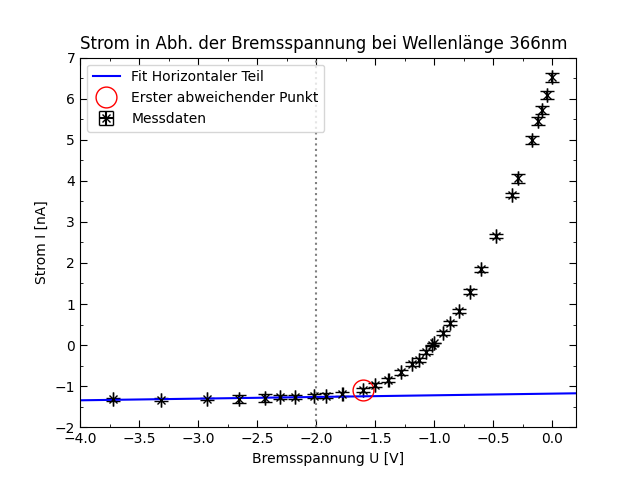
\includegraphics[width=1\linewidth]{../Images/Planck366.png}
   			 \caption{Bremsspannung für $\lambda = 366 \, nm$}
   			 \label{Img:Brems366}
		\end{figure}
		Aus diesen Messungen ergibt sich:
		\begin{table}[H]          %so funktionieren die Tabellen in LaTeX
		\centering
		\begin{tabular}{c|c}

		$\lambda \, [nm]$  	& $U_B \, [V]$\\
		\hline
  		$366$				& $(-0.952 \pm 0.024)$\\
		$405$				& $(-0.7841 \pm 0.0097)$\\
		$436$				& $(-0.631 \pm 0.010)$\\
		$546$				& $(-0.388 \pm 0.012)$\\
		$578$				& $(-0.31 \pm 0.11)$
		\end{tabular}  
		\caption{Kniespannungen für die unterschiedlichen Wellenlängen}  %siehe Graphik: Beschriftung
		\label{Tab:WellenU}                             %siehe Graphik: zum Zitieren
		\end{table}
		\noindent Mit der Lichtgeschwindigkeit ($c = 299792458 \, \frac{m}{s}$) kann nun aus
		\begin{equation*}
			\nu = \frac{c}{\lambda}
		\end{equation*}
		Die Lichtfrequenz berechnet werden. 
		Mit (\ref{eq:EinsteinGleichung}) kann wie in \ref{sec:TheoPlanck} erklärt die Plankkonstante bestimmt werden.
		\begin{figure}[H]
			\centering
			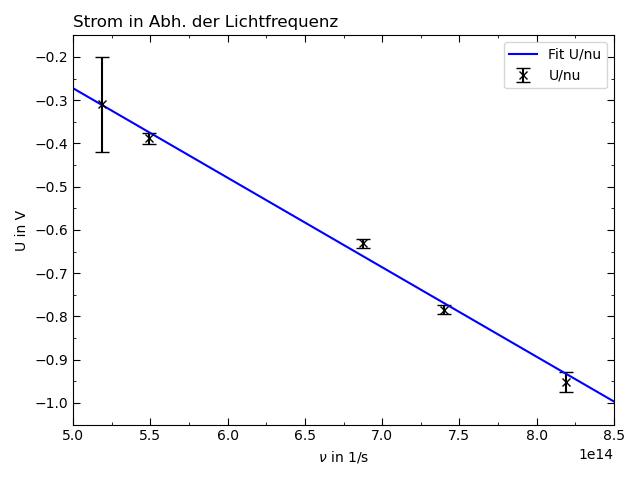
\includegraphics[width=1\linewidth]{../Images/U_nu.png}
			\caption{CAPTION}
			\label{Img:Inu}
		\end{figure}
		\noindent Der Fit in Abb.\ref{Img:Inu} steigt mit $m = (-2.069 \pm 0.073)\cdot 10^{-15} \, V s$ an.
		Aus
		\begin{equation*}
			h = m \, e
		\end{equation*}
		(Gleichung resultiert aus (\ref{eq:EinsteinGleichung})) berechnet sich $h = (-3.32 \pm 0.12)\cdot 10^{-35} \, J s$.
\section{Zusammenfassung}

\begin{thebibliography}{}    %so wird das Literaturverzeicnis erstellt
\bibitem{BipBop}
	\url{https://www.physik.uni-wuerzburg.de/fileadmin/11000000/03_Studium/02_Bachelor/Grundpraktikum/_imported/fileadmin/11016800/Modulbeschreibungen/C-Modul/Versuch_41_ueberarbeitet.pdf}, besucht am 20.11.2025
\bibitem{Lichtgeschwindigkeit}
	\url{https://physics.nist.gov/cgi-bin/cuu/Value?c}, besucht am 18.11.2025 um 16.29 Uhr
\bibitem{Koaxialkabel1}
	\url{https://docs.rs-online.com/75d1/A700000011339821.pdf}, besucht am 20.11.2025 um 00.59 Uhr
\bibitem{Koaxialkabel2}
	\url{https://www.auer-kunststofftechnik.de/pdf/Technisch.Datenblatt\%20PE\%20-LD\%20natur\%2070093.pdf}, besucht am 20.11.2025 um 08:05 Uhr
\end{thebibliography}

\end{document}